\documentclass[main.tex]{subfiles}
\begin{document}

\section{Photon statistics}

\subsection{Background}

Just like the classical Maxwell equations take the form of a classical harmonic oscillator, a single mode of the photon field can be described as a quantum harmonic oscillator.

We wish to describe photon statistics pertaining to a laser beam, so we are justified in fixing the \(\omega \) of the light.

\textbf{Coherent light} is the closest quantum approximation we can find for the monochromatic plane wave solution. A coherent state \(\ket{\alpha } \) can be defined to be an eigenstate of the annihilation operator \(\hat{a}\): \(\hat{a} \ket{\alpha } = \alpha \ket{\alpha }\). 

We can write these states in terms of the Fock number states \(\ket{n}\) as: 
%
\begin{align}
\ket{\alpha } = \exp(- \frac{\abs{\alpha }^2}{2}) 
\sum _{n} \frac{\alpha^{n}}{n!} \ket{n}
\,,
\end{align}
%
and the expectation value of the electric field in a certain direction is oscillatory as expected: 
%
\begin{align}
\ev{\hat{E}_x}{\alpha } = i \sqrt{\frac{\hbar \omega }{ 2 \epsilon_0 V}} \qty( \alpha  e^{i k_\mu x^{\mu }} - \alpha^{*} e^{-i k_\mu x^{\mu }} )
\,,
\end{align}
%
where we use the mostly plus metric convention, \(\epsilon_0 \) is the vacuum dielectric permittivity and \(V\) is the volume of the ``box'' in which the field is contained. 
The average number of photons is given by \(\overline{n} = \abs{\alpha }^2\), and with this we can describe the statistics of the number of photons we would find in a certain region: it follows a Poisson distribution, 
%
\begin{align}
\abs{\braket{\alpha }{n}}^2 = \frac{e^{-\overline{n}} \overline{n}^{n}}{n!}
\,.
\end{align}

\textbf{Thermal light}, on the other hand, has the distribution we would expect to see if, for instance, we had a bath of atoms in thermal equilibrium with radiation and a transition with energy \(\hbar \omega \)\cite[section 14.4]{salehFundamentalsPhotonics}.

The distribution describing this situation is the Boltzmann one: 
%
\begin{align}
\mathbb{P} (E_n) \propto \exp( - \frac{E_n}{k_B T})
\,,
\end{align}
%
and in our case, using \(E_n = n \hbar \omega \) and the fact that the mean photon number is given by 
%
\begin{align}
\overline{n} = \frac{1}{\exp( \hbar \omega  / k_B T) - 1}
\,,
\end{align}
%
we can write this as 
%
\begin{align}
\mathbb{P}(n) = \frac{1}{\overline{n} +1} \qty(\frac{\overline{n}}{\overline{n}+1})^{n}
\,.
\end{align}

In quantum terms, this is a \emph{completely mixed} state, a classical probabilistic mixture of the number states \(\ket{n}\), described by the density matrix 
%
\begin{align}
\rho _{\text{thermal}} = \sum _{n} \mathbb{P}(n) \dyad{n} 
\,.
\end{align}

Since the number states \(\ket{n}\) have zero expectation value for the electric field, here also we find \(\expval{\hat{E}_x}_{\text{thermal}} = 0\). 

\subsection{Experimental setup}

We create a setup which allows us to conveniently create coherent and thermal states at will.

We start from a laser: the light it produces is coherent, and thus obeys Poisson statistics. 
We bounce this laser off a disk, which is covered in sandpaper. The shape of the apparatus is quite simple; it is shown in figure \ref{fig:sandpaper}.  
The sandpaper is reflective, so as long as the disk is stationary we expect the statistics of the light to be preserved. We will see that this is experimentally verified. 

\begin{figure}[ht]
\centering


\tikzset{every picture/.style={line width=0.75pt}} %set default line width to 0.75pt        

\begin{tikzpicture}[x=0.75pt,y=0.75pt,yscale=-1,xscale=1]
%uncomment if require: \path (0,300); %set diagram left start at 0, and has height of 300

%Shape: Rectangle [id:dp22021547584457224] 
\draw   (32,82) -- (102,82) -- (102,122) -- (32,122) -- cycle ;
%Shape: Wave [id:dp04968334570050592] 
\draw  [dash pattern={on 4.5pt off 4.5pt}] (103,100.7) .. controls (107.08,104.03) and (110.98,107.2) .. (115.5,107.2) .. controls (120.02,107.2) and (123.92,104.03) .. (128,100.7) .. controls (132.08,97.37) and (135.98,94.2) .. (140.5,94.2) .. controls (145.02,94.2) and (148.92,97.37) .. (153,100.7) .. controls (157.08,104.03) and (160.98,107.2) .. (165.5,107.2) .. controls (170.02,107.2) and (173.92,104.03) .. (178,100.7) .. controls (182.08,97.37) and (185.98,94.2) .. (190.5,94.2) .. controls (195.02,94.2) and (198.92,97.37) .. (203,100.7) .. controls (207.08,104.03) and (210.98,107.2) .. (215.5,107.2) .. controls (220.02,107.2) and (223.92,104.03) .. (228,100.7) .. controls (232.08,97.37) and (235.98,94.2) .. (240.5,94.2) .. controls (245.02,94.2) and (248.92,97.37) .. (253,100.7) .. controls (257.08,104.03) and (260.98,107.2) .. (265.5,107.2) .. controls (270.02,107.2) and (273.92,104.03) .. (278,100.7) .. controls (282.08,97.37) and (285.98,94.2) .. (290.5,94.2) .. controls (295.02,94.2) and (298.92,97.37) .. (303,100.7) .. controls (307.08,104.03) and (310.98,107.2) .. (315.5,107.2) .. controls (319.02,107.2) and (322.16,105.28) .. (325.3,102.86) ;
%Shape: Ellipse [id:dp2897372001959284] 
\draw   (354.86,88.89) .. controls (365.17,99.2) and (368.73,112.35) .. (362.82,118.27) .. controls (356.9,124.18) and (343.75,120.62) .. (333.44,110.31) .. controls (323.13,100) and (319.57,86.85) .. (325.48,80.93) .. controls (331.4,75.02) and (344.55,78.58) .. (354.86,88.89) -- cycle ;
%Shape: Wave [id:dp798169784205734] 
\draw  [dash pattern={on 4.5pt off 4.5pt}] (338.58,118.55) .. controls (335.34,122.64) and (332.25,126.55) .. (332.27,131.08) .. controls (332.29,135.6) and (335.4,139.49) .. (338.67,143.55) .. controls (341.95,147.62) and (345.06,151.5) .. (345.08,156.03) .. controls (345.09,160.55) and (342.01,164.46) .. (338.77,168.55) .. controls (335.53,172.64) and (332.45,176.55) .. (332.46,181.08) .. controls (332.48,185.6) and (335.59,189.49) .. (338.87,193.55) .. controls (342.14,197.61) and (345.25,201.5) .. (345.27,206.03) .. controls (345.28,208.94) and (344.01,211.6) .. (342.23,214.21) ;
%Shape: Chord [id:dp4480069197470371] 
\draw   (378.22,209.27) .. controls (380.01,212.87) and (381,216.84) .. (381,221) .. controls (381,237.57) and (365.33,251) .. (346,251) .. controls (326.67,251) and (311,237.57) .. (311,221) .. controls (311,216.84) and (311.99,212.87) .. (313.78,209.27) -- cycle ;

% Text Node
\draw (40,93) node [anchor=north west][inner sep=0.75pt]   [align=left] {LASER};
% Text Node
\draw (316,218) node [anchor=north west][inner sep=0.75pt]   [align=left] {Detector};
% Text Node
\draw (292,51) node [anchor=north west][inner sep=0.75pt]   [align=left] {Sandpaper disk};


\end{tikzpicture}
\caption{Sandpaper setup.}
\label{fig:sandpaper}
\end{figure}

The sandpaper disk is then spun up: because of the roughness, the exact location from which the light bounces off changes moment by moment, so the electric field is \emph{scrambled}: it loses coherence, and its expectation value over a sufficient period of time becomes zero, which as we saw is a characteristic of thermal light.

\subsection{Data preparation}

We have two data acquisitions, labelled based on the distribution we expect from them: ``coherent'' and ``thermal''. 
The former is taken with the disk being kept stationary, the latter is taken with the moving disk. 

The data from the timetagger is a series of arrival times, in units of its resolution, which is of \SI{80.955}{ps}. 

In order to recover the statistics for a certain acquisition, we select a window size \(w\); divide the total acquisition time into intervals of size \(w\), and count how many photons were detected in each interval.

We then make a histogram of these numbers: after normalization, this procedure yields a probability distribution \(\mathbb{P}_w(n)\).

\subsection{Analysis}

The first kind of analysis one can do is to fit the corresponding distribution to the data. What should we assign as a window size? 

\begin{figure}[ht]
\centering
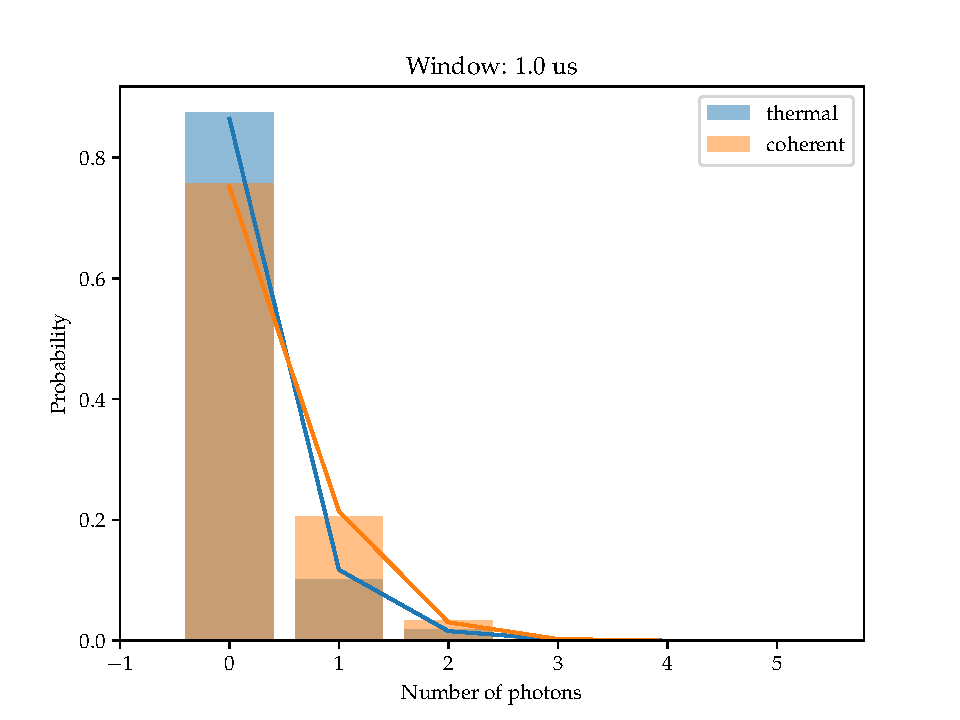
\includegraphics[width=\textwidth]{figures/1.0us}
\caption{Probability of seeing a certain number of photons per window of \SI{1}{\micro s}.}
\label{fig:1.0us}
\end{figure}

\begin{figure}[ht]
\centering
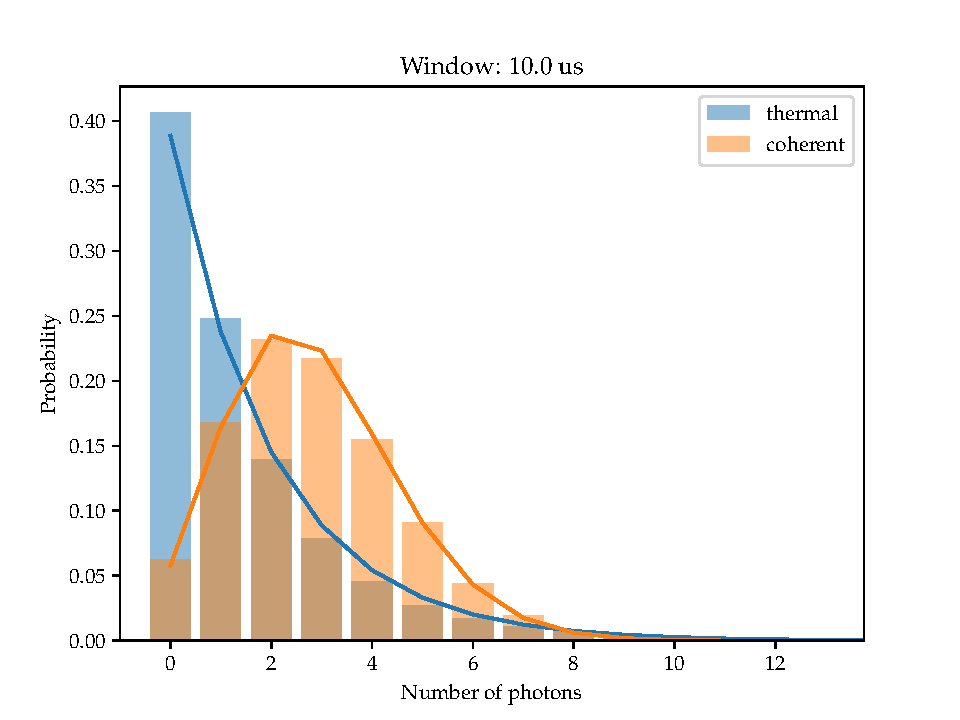
\includegraphics[width=\textwidth]{figures/10.0us}
\caption{Probability of seeing a certain number of photons per window of \SI{10}{\micro s}.}
\label{fig:10.0us}
\end{figure}

\begin{figure}[ht]
\centering
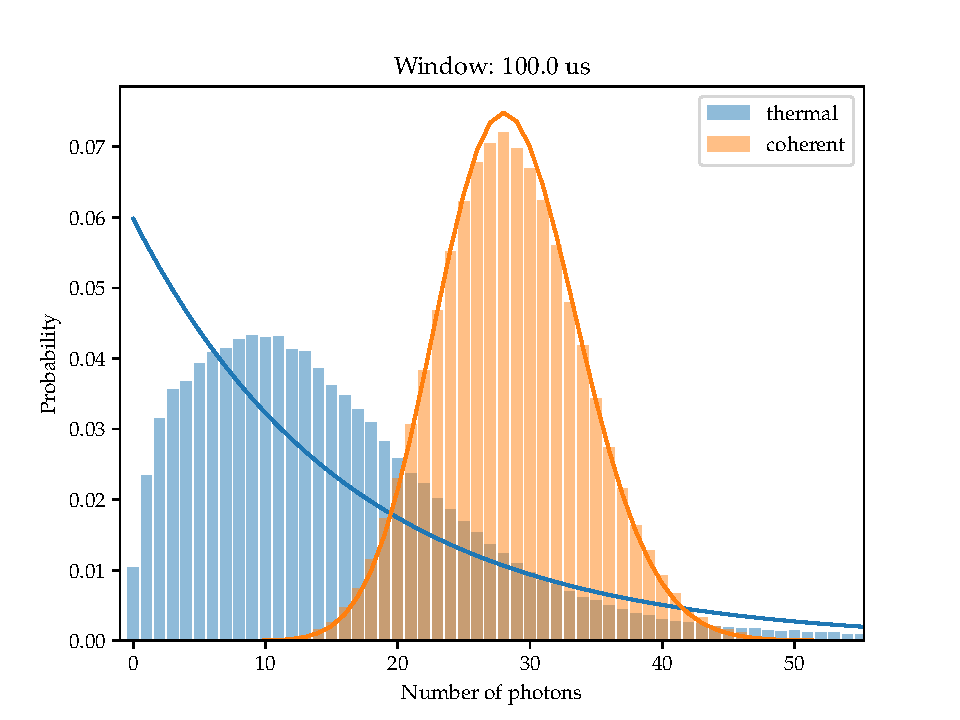
\includegraphics[width=\textwidth]{figures/100.0us}
\caption{Probability of seeing a certain number of photons per window of \SI{100}{\micro s}.}
\label{fig:100.0us}
\end{figure}

In figures \ref{fig:1.0us}, \ref{fig:10.0us} and \ref{fig:100.0us} we show the plots we find with a few different window sizes. The histogram is from the data, the line comes from the theoretical distribution computed by fixing the mean to be equal to that of the data.

We can see that with window sizes of the order of \SI{10}{\micro s} the distribution is close to the theoretical one and the coherent and thermal ones look quite different; for smaller windows we start to rarely see even a single photon per window, for larger ones the mode of the ``thermal'' distribution shifts from zero.

In order to understand this behaviour more specifically, we can compare the first moments of the distributions to the theoretical ones: we can compute the mean
%
\begin{align}
\overline{n} = \sum _{n} \mathbb{P}(n) n
\,,
\end{align}
%
the variance 
%
\begin{align}
\sigma^2 = \sum _{n} \mathbb{P}(n) (n - \overline{n})^2
\,,
\end{align}
%
the normalized skewness 
%
\begin{align}
\text{skewness} = \frac{1}{\sigma^3} \sum _{n} \mathbb{P}(n) (n - \overline{n})^3
\,,
\end{align}
%
and the normalized kurtosis 
%
\begin{align}
\text{kurtosis} = \frac{1}{\sigma^4} \sum _{n} \mathbb{P}(n) (n - \overline{n})^4
\,.
\end{align}

For each window size \(w\) we compute the moments of the experimental distribution, and the corresponding ones for the theoretical distribution computed by fixing the mean to be the experimental one.
The results, for window sizes varying from \SI{10}{ns} to approximately \SI{3}{ms}, are shown in figure \ref{fig:photon_statistics}. Beyond the moments, the mode is also shown. 

\begin{sidewaysfigure}[ht]
    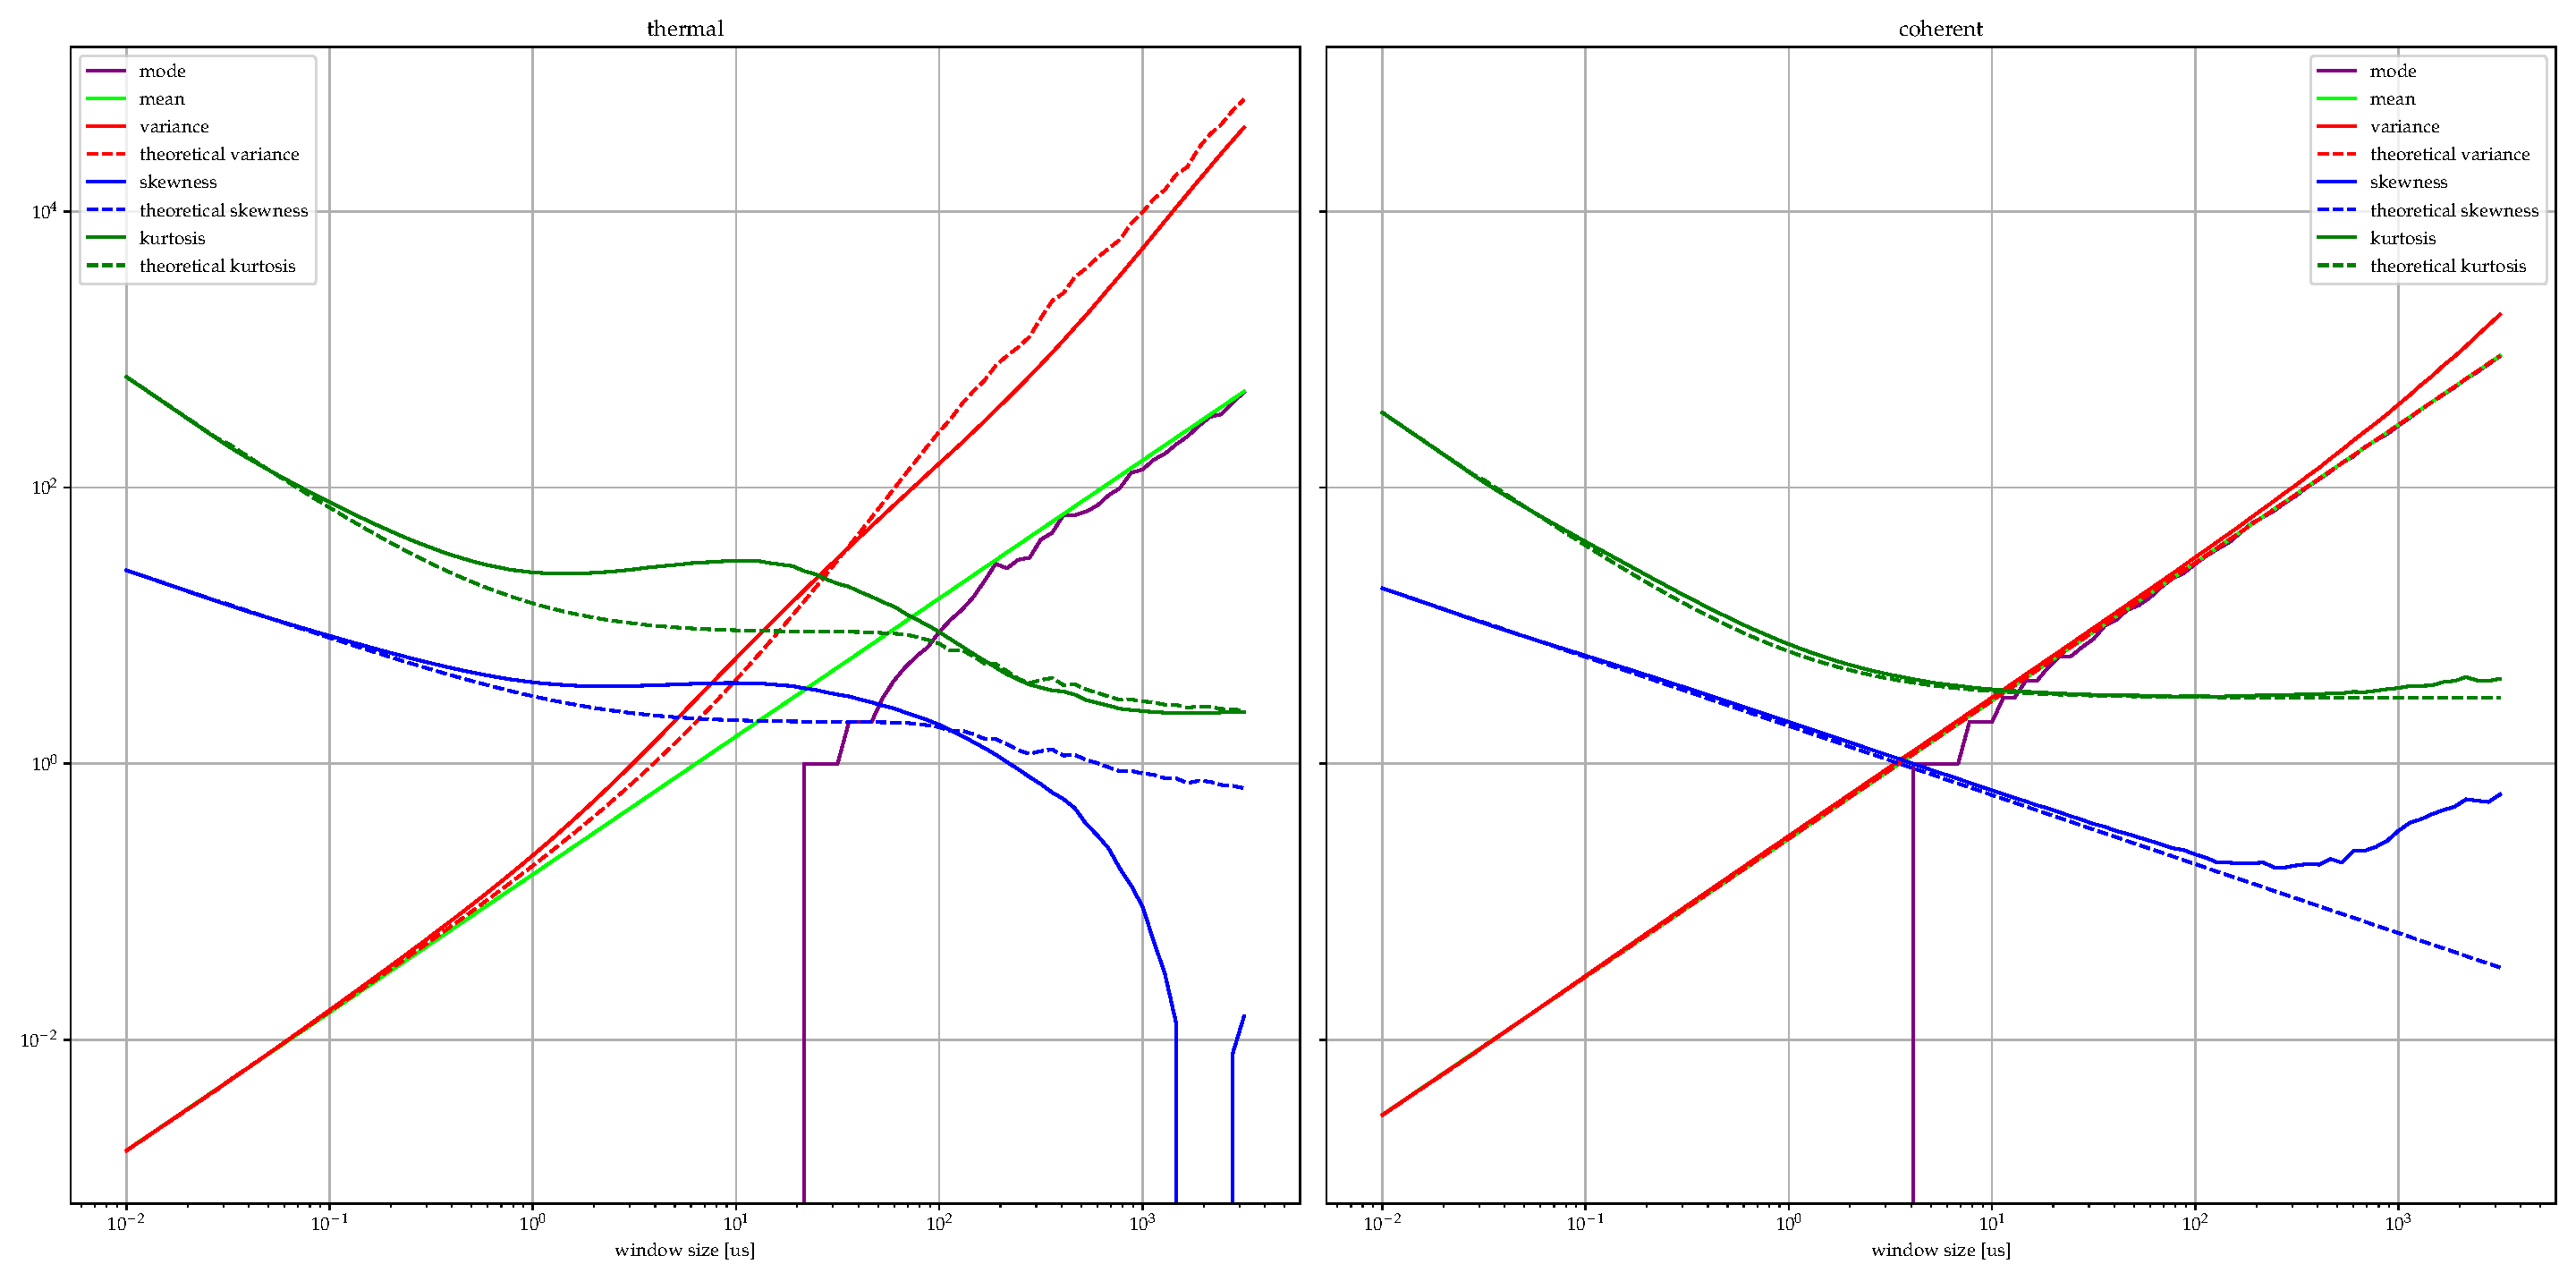
\includegraphics[width=\textwidth]{figures/photon_statistics.pdf}
    \caption{Photon statistics.}
    \label{fig:photon_statistics}
\end{sidewaysfigure}

We can see that the results trace quite well with the theoretical ones for the coherent case, especially for window sizes of \SI{100}{\micro s}: this is to be expected, and it gives us a way to estimate the coherence length of the LASER. 

This is not the case for the thermal state, but it is not a terrible approximation. At \SI{10}{\micro s} the mean, variance and mode are good, the skewness and kurtosis are a bit off --- these higher moments are more influenced by noise at higher photon numbers, so it is understandable that they are more difficult to adjust. 

It is understandable that the distribution does not come out to be exactly thermal: what the rotating sandpaper disk does is to effectively remove any kind of phase coherence, and therefore to enforce the expectation value of the electric field to be zero. 
Any mixture of number states, however, has this property! 
The incoming state is still coherent, and with this setup some coherence ``shines through'': perhaps with more than one rotating disk the state might have enough interactions with the environment to thermalize --- this has not fully happened in our case. 

\end{document}